\documentclass[12pt]{article}
\usepackage[a4paper, margin=.30in]{geometry}
\usepackage{graphicx ,
            wrapfig,
            xcolor, 
            enumerate,
            amsmath,fontenc, makecell
            }

\newcommand\headerMe[2]{\noindent{}#1\hfill#2}
\renewcommand{\thesection}{\Roman{section}}

\author{Zakaria HAOUZAN}
\date{\today}

\begin{document}
% headers --------------
\headerMe{Matière : Physique-Chimie}{Professeur : Zakaria HAOUZAN}\\
\headerMe{Unité : La Mécanique}{Établissement : Lycée SKHOR qualifiant}\\
\headerMe{Niveau : TCS}{Heure : 4H}\\

% ------Content ________
\begin{center}
    \Large{Leçon $N^{\circ}6$: \color{red} Equilibre d’un corps solide soumis à 3 forces }
\end{center}

\begin{wrapfigure}{r}{0.2\textwidth}

\includegraphics[width=0.2\textwidth]{./img/img00.jpg}
\end{wrapfigure}


\section{Situation problème : }
Le schéma ci-contre représente un alpiniste qui est en équilibre sous
l’action de 3 forces : son poids $\vec{P}$ , la réaction $\vec{R}$ , et la tension de la
corde $\vec{T}$
\\ - Quelles sont les conditions d’équilibre d’un corps solide
soumis à 3 forces ?
\\ - Comment utiliser ses conditions pour déterminer les intensités
de quelques forces, et aussi les valeurs d’autres grandeurs ?



\section{Conditions d’équilibre d'un corps solide sous l'action de trois forces non parallèles : }
\subsection{ Etude de l’équilibre d’un solide soumis à trois forces non parallèles  }
\subsubsection{Activité expérimentale N°1 }
 
\begin{wrapfigure}{r}{0.3\textwidth}
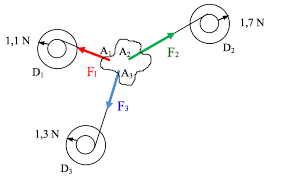
\includegraphics[width=0.3\textwidth]{./img/img01.png}
\end{wrapfigure}

On réalise l’équilibre d’une plaque très légère avec trois dynamomètres, comme l’indique le schéma ci-contre : 
\\1 - Faire l’inventaire des forces appliquées sur la plaque, puis déterminer la force qu’on peut négliger son
intensité devant l'intensité des autres
\\2 - Tracer les lignes d’action des forces appliquées sur la plaque.
Que constatez-vous sur ses lignes d’action ?
\\3 - Copier le schéma ci-contre sur votre cahier, et tracer les forces
appliquées sur la plaque en choisissant une échelle
\\4 - Tracer la ligne polygone des forces appliquées sur la plaque.
Que peut-on dire sur la somme vectorielle des forces
appliquées sur la plaque ?
\\5 - Conclure les conditions d'équilibre nécessaires d’un corps
solide soumis à trois forces non parallèles.
\subsubsection{ Exploitation: }
 1 . Le système étudié est la plaque {S} , Le bilan des forces exercées sur la plaque
 \\$F_1$ la force exercée par le dynamomètre D1
 \\ $F_2$ la force exercée par le dynamomètre D2
 \\ $F_3$ la force exercée par le dynamomètre D3
 \\P  le poids de la plaque : Puisque la masse de la plaque est néglieable alors son poids est néglieable devant
les intensités des autres forces F1 = 2N et F2= 2N et F3 = 1N
Donc on peut dire que la plaque S est en équilibe sous l’action de trois forces (F1, F2, F3)non parallèles
\\Les caractéristiques des forces : 
\begin{center}
  \begin{tabular}{|c|c|c|c|c|}
    \hline
    force & Point d’application & Droite d’action & Sens &intensité \\\hline
    $F_1$ & $A_1$               & \makecell{La droite confondue avec \\ le fil du dynamomètre D1}  & De A1 vers D  & F1 = 2 N  \\\hline
    $F_2$ & $A_2$               & \makecell{ La droite confondue avec \\ le fil du dynamomètre D2 } & De A2 vers D  & F1 = 2 N  \\\hline
    $F_3$ & $A_3$               & \makecell{La droite confondue avec\\ le fil du dynamomètre D3}& De A3 vers D  & F1 = 1 N  \\\hline

  \end{tabular}
\end{center}

2 . On remarque les trois lignes d’action se coupent en un même point : on dit que les droites d’action des
trois forces $\vec{F_1}$,$\vec{F_2}$ et $\vec{F_3}$ sont concourantes

Après avoir réalisé l’équilibre de la plaque, l’expérience montre que les trois forces $\vec{F_1}$,$\vec{F_2}$ et $\vec{F_3}$ non parallèle sont situées dans un même plan, on dit que les trois forces $\vec{F_1}$,$\vec{F_2}$ et $\vec{F_3}$ sont coplanaires .

3 . On utilise l’échelle suivante : 1 cm = 1 N

4 .\underline{ Méthode graphique( ligne polygonale) :} On représente la somme vectorielle de trois forces $\vec{F_1}$,$\vec{F_2}$ et $\vec{F_3}$. on obtient une ligne polygonale
fermée. Donc on constate que la somme vectorielle de ces trois forces $\vec{F_1}$,$\vec{F_2}$ et $\vec{F_3} $ est égale au
vecteur nul : \[\vec{F_1} + \vec{F_2} +  \vec{F_3} = \vec{0} \]

5 . les conditions d’équilibre :  Pour qu’un solide soit en équilibre sous l’action de trois forces non parallèles, il faut que :

-Les droites d’action des trois forces soient coplanaires et concourantes.

-la somme vectorielle des forces soit égale au vecteur nul

\subsection{Conclusion : }
Lorsqu’un solide soumis à trois forces $\vec{F_1}$,$\vec{F_2}$ et $\vec{F_3}$ non parallèles est en équilibre , alors :  
 Pour qu’un solide soit en équilibre sous l’action de trois forces non parallèles, il faut que :
 la somme vectorielle des trois forces est égale au vecteur nul $ \vec{F_1} + \vec{F_2} +  \vec{F_3} = \vec{0}$  u la ligne polygonale des trois forces est fermée . cette condition est nécessaire pour que le centre d’inertie G
du corps soit au repos 

les droites d’action des trois forces sont coplanaires et concourantes. cette condition est nécessaire pour
l’absence de rotation du corps autour de lui-même, sil la première condition est vérifiée.

\section{Application : méthode géométrique, méthode analytique }
 
\begin{wrapfigure}{r}{0.4\textwidth}
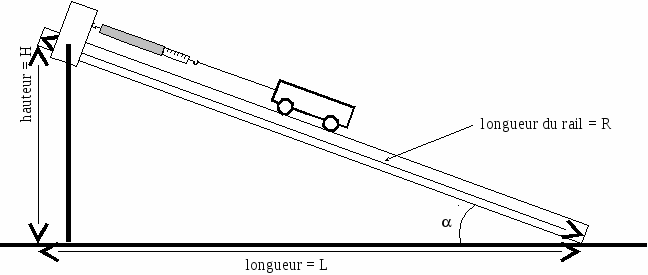
\includegraphics[width=0.4\textwidth]{./img/img03.png}
\end{wrapfigure}

\subsection{ Equilibre d’un solide sur un plan incliné: cas d’un contact sans frottement}
\subsubsection{Activité expérimentale N°2 :étude de l’équilibre d’un solide sur un plan incliné  }

 Un solide S de masse m = 360 g maintenu en équilibre, sur un plan incliné ($\pi$) d’un angle $\alpha = $25° , grâce à un dynamomètre. Tel que T = 1,5 N.
 
 1. Déterminer le système étudié
 
 2. Faire l’inventaire des forces appliquées sur le solide (S)

 3. Déterminer par deux méthodes différentes : géométrique et
arithmétique (analytique), la réaction $\vec{R}$ du plan sur le corps solide S
(les caractéristiques de $\vec{R}$ ) . Conclure

\subsubsection{Interprétation : }

Le système étudié est le corps ( S )

Le bilan des forces exercées sur la masse marquée:
\\$\vec{P}$ : Le poids du corps ( S )
\\$\vec{T}$ : La force exercée par le dynamomètre
\\$\vec{R}$ : La réaction du plan incliné ( la force exercée par le plan incliné sur le corps ( S) )

Déterminons $\vec{R}$ La réaction du plan incliné par deux méthodes : géométrique et analytique

\subsubsection{Méthode géométrique / méthode graphique : }
Le corps est en équilibre sous l’action de trois forces $\vec{P}$ ,$\vec{T}$ et $\vec{R}$ donc $\vec{P} + \vec{R} + \vec{T} = \vec{0}$ ,
 alors la ligne polygonale est fermée ( la dynamique des forces est un triangle fermé ) .

La connaissance des caractéristiques de $\vec{P}$ ,$\vec{T}$ et $\vec{R}$  permet de tracer la ligne polygonale fermée et par
conséquent, on peut déterminer les caractéristiques de $\vec{R}$

Donc pour tracer la somme des forces , on commence par $\vec{T}$ qui a une droite d’action incliné d’un angle
$\alpha$ = 25° puis $\vec{P}$ le poids qui est perpendiculaire au plan  et dirigé vers le bas , alors pour déterminer $\vec{R}$
( les caractéristiques de $\vec{R}$ ) , on ferme le triangle ( Voir le schéma )
 
\begin{center}
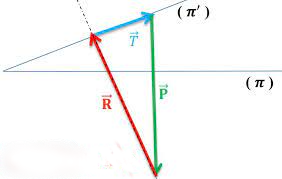
\includegraphics[width=0.3\textwidth]{./img/img04.png}
\end{center}

Pour représenter les forces on utilise l’échelle suivante : 1.5 N = 2cm
\\Pour $\vec{T}$ : on a  T=1.5N $\rightarrow$ 2cm
\\Pour $\vec{P}$ : P = mg = 3.6N $\rightarrow$ 4.8cm

Remarque : On remarque que la direction de $\vec{R}$ est perpendiculaire au plan incliné  , cela signifie que le contact entre le solide et le plan se fait sans frottement .

Les caractéristiques de $\vec{R} : $
\\Le point d’application : le point A
\\La droite d’action : droite perpendiculaire au plan incliné et passant par le point A
\\Le sens : vers le haut
\\L’intensité : on peut déterminer R L’intensité de $\vec{R}$ par deux méthodes 
\begin{enumerate}
  \item Méthode 1 : L’échelle : On a R = 4.36cm donc R=3.27N
  \item théorème de Pythagore : D’après le théorème de Pythagore on a  $$R^2 + T^2 = P^2$$
    donc $$R = \sqrt{R^2 + T^2}$$
\end{enumerate}

\subsubsection{Méthode Arithmétique ou Analytique : (projection des forces sur les axes d’un repère)}

Cette méthode consiste sur la projection de la relation $\sum{\vec{F}_{ext}}$ sur les axes d’un repère $ R(O, \vec{i}, \vec{j}, \vec{k})$

considérons un repère orthonormé $ R(O, \vec{i}, \vec{j}, \vec{k})$ tel que son origine O est confondu avec le centre d’inertie G
du solide ( S ) ( voir le schéma ci-contre )

Puisque le corps est en équilibre sous l’action de trois forces $\vec{P}$ ,$\vec{T}$ et $\vec{R}$ 
alors  $\vec{P} + \vec{R} + \vec{T} = \vec{0}$

On projette cette relation sur les axes ( Ox ) et ( Oy ) ,et On obtient :

$$\begin{cases}
  P_x + T_x + R_x = 0\\
  P_y + T_y + R_y = 0
\end{cases}
$$
D’après le schéma On a : 

$\begin{cases}
  P_x = -Psin\alpha\\
  P_y = -Pcos\alpha
\end{cases}
$ et 
$\begin{cases}
  T_x = T\\
  T_y = 0
\end{cases}
$ donc 
$\begin{cases}
  -Psin\alpha + T + R_x = 0\\
  -Pcos\alpha + 0 + R_y = 0\\
\end{cases}
$
alors 
$\begin{cases}
  R_x = Psin\alpha - T \\
  R_y = Pcos\alpha\\
\end{cases}
$

A.N
$
\begin{cases}
  R_x = 0 N \\
  R_y = 3.26N\\
\end{cases}
$
Or R = $\sqrt{R_x^2 + R_y^2}$ d’où R = 3.26N

D’autre part, On sait que $\vec{R} = \vec{R_x}  + \vec{R_y}$ donc $\vec{R}$ =$\vec{R_y}$ puisque $\vec{R_x} = \vec{0}$, alors la réaction $\vec{R}$ est
perpendiculaire au plan incliné , cela signifie que le contact entre le solide et le plan se fait sans
frottement . ( même résultat que celui obtenu dans la méthode précédente )

\subsection{Equilibre d’un solide sur un plan incliné: Cas d’un contact avec frottement }
\subsubsection{Activité expérimentale N°3 : Force de frottement, Angle de frottement, coefficient de frottement  }
Un solide ( s) , de masse m = 5 Kg , est en équilibre avec frottement sur un plan incliné d’un angle $\alpha $= 60°
par rapport à la verticale i

1. Faire le bilan des forces extérieures agissant sur le solide et les
dessiner sur le schéma de la figure

2. En appliquant la condition d’équilibre, déterminer :
  
  a. L’intensité R de la réaction du plan incliné sur le solide
 
  b. La composante normale RN de la réaction $\vec{R}$

  c. La composante tangentielle RT de la réaction $\vec{R}$ (a valeur de la
force de frottement)

3. Calculer K le coefficient de frottement

4. Déduire $\phi$ l’angle de frottement


\subsubsection{Interprétation :}

1. Le bilan des forces extérieurs exercées sur le solide ( S ) :$ \vec{P}$ -> Le poids du solide et $\vec{R}$ :La Réaction du plan incliné avec   $\vec{R} = \vec{R_N} + \vec{R_T}$

$\vec{R_N}$ : La composante normale
$\vec{R_T} $ : La composante tangentielle ou La force de
frottement  $\vec{f} (\vec{R_T} =\vec{f}) $

\begin{itemize}
    \item  $\vec{R} = \vec{R_N} + \vec{R_T}$
    \item  $\varphi$: l’angle de frottement
    \item K = $tg\varphi = \frac{R_T}{R_N}$ Coefficient de frottement 
\end{itemize}
Représentation des forces $\vec{{P}} et\vec{R}$ 
le corps ( S ) est en équilibre sous l’action de deux forces $\vec{{P}} et\vec{R}$ alors $\vec{P} + \vec{R} = \vec{0}$
cela signifie
que les deux forces ont la même droite d’action, des sens opposés et la même intensité
R = P =mg =50N

On prend 10 N =  1 cm comme l’échelle pour représenter ces deux forces 

2. Etude de l’équilibre du solide ( S) sur le plan incliné sous l’action de deux forces :
 
 a - Le corps ( S ) est en équilibre sous l’action de deux forces $\vec{{P}} et\vec{R}$ alors R = P = 50N

 b - Pour déterminer RN La composante normale de la réaction $\vec{R}$ , on projette la relation $\vec{P} + \vec{R} = \vec{0}$ sur (Ox) et (Oy) : 
$$\begin{cases}
  P_x + R_x = 0\\
  P_y + R_y = 0
\end{cases}
$$
D’après le schéma On a : 

$\begin{cases}
  P_x = Psin\alpha\\
  P_y = -Pcos\alpha
\end{cases}
$ et
$\begin{cases}
  R_x = -R_T \\
  R_y = R_N
\end{cases}
$
ce qui donne
$\begin{cases}
  R_T = -P_x  = m.g.sin\alpha = 25N\\
  R_N = -P_y = -m.g.cos\alpha = 43.3N
\end{cases}
$
\\On constate que R = $\sqrt{R_N^2 + R_T^2}$

Calculons K le coefficient de frottement : K = $tg\varphi = frac{R_T}{R_N} = 0.58$

Déterminons $\varphi$ l’angle de frottement :

D’après la question précédente , on a $\varphi = tg^{-1}(0.58)$ donc $\varphi = 30^\circ$

\end{document}
